%! Tex program = xelatex   
\documentclass{article}
\usepackage{graphicx,subfig}
\usepackage[left=2cm, right=2cm, lines=45, top=0.8in, bottom=0.7in]{geometry}
\usepackage{xeCJK}
\usepackage{amsmath}
\usepackage{booktabs} %表格
\usepackage{tikz}
\usepackage{graphics}
\usepackage{xcolor} 
\usepackage{tikz} 
\usepackage{svg}
\usetikzlibrary{arrows,shapes,chains}
\setmainfont{Times New Roman}
\setCJKmainfont{Songti SC}
\setCJKfamilyfont{song}{Songti SC}
\renewcommand{\baselinestretch}{1.5} %行间距
%-----------------------伪代码------------------
\usepackage{algorithm}  
\usepackage{algorithmicx}  
\usepackage{algpseudocode}  
\floatname{algorithm}{Algorithm}  
\renewcommand{\algorithmicrequire}{\textbf{Input:}}  
\renewcommand{\algorithmicensure}{\textbf{Output:}} 
\usepackage{lipsum}  
\makeatletter
\newenvironment{breakablealgorithm}
  {% \begin{breakablealgorithm}
  \begin{center}
     \refstepcounter{algorithm}% New algorithm
     \hrule height.8pt depth0pt \kern2pt% \@fs@pre for \@fs@ruled
     \renewcommand{\caption}[2][\relax]{% Make a new \caption
      {\raggedright\textbf{\ALG@name~\thealgorithm} ##2\par}%
      \ifx\relax##1\relax % #1 is \relax
         \addcontentsline{loa}{algorithm}{\protect\numberline{\thealgorithm}##2}%
      \else % #1 is not \relax
         \addcontentsline{loa}{algorithm}{\protect\numberline{\thealgorithm}##1}%
      \fi
      \kern2pt\hrule\kern2pt
     }
  }{% \end{breakablealgorithm}
     \kern2pt\hrule\relax% \@fs@post for \@fs@ruled
  \end{center}
  }
\makeatother
%------------------------代码-------------------
\usepackage{xcolor} 
\usepackage{listings} 
\usepackage{fontspec}
\newfontfamily\menlo{Menlo}
\setmonofont[Mapping={}]{Monaco} 
\definecolor{mygreen}{rgb}{0,0.6,0}
\definecolor{mygray}{rgb}{0.5,0.5,0.5}
\definecolor{mymauve}{rgb}{0.58,0,0.82}
\lstset{ %
backgroundcolor=\color{white},   % choose the background color
basicstyle=\footnotesize\ttfamily,        % size of fonts used for the code
columns=fullflexible,
breaklines=true,                 % automatic line breaking only at whitespace
captionpos=b,                    % sets the caption-position to bottom
tabsize=4,
commentstyle=\color{mygreen},    % comment style
escapeinside={\%*}{*)},          % if you want to add LaTeX within your code
keywordstyle=\color{blue},       % keyword style
stringstyle=\color{mymauve}\ttfamily,     % string literal style
frame=single,
rulesepcolor=\color{red!20!green!20!blue!20},
numbers=left,
 numberstyle=\tiny\menlo
% identifierstyle=\color{red},
% language=c++,
}
\begin{document}
\title{CNN实验报告}
\author{朱浩泽 1911530}
\maketitle
\section{老师提供的基础CNN网络}
\large
\subsection{网络结构}
我们通过 Pycharm 软件的 python 控制台查看运行时的变量,可以看到网络结构如下:
\begin{lstlisting}[language=c++]
Net(
  (conv1): Conv2d(3, 6, kernel_size=(5, 5), stride=(1, 1))
  (pool): MaxPool2d(kernel_size=2, stride=2, padding=0, dilation=1, ceil_mode=False)
  (conv2): Conv2d(6, 16, kernel_size=(5, 5), stride=(1, 1))
  (fc1): Linear(in_features=400, out_features=120, bias=True)
  (fc2): Linear(in_features=120, out_features=84, bias=True)
  (fc3): Linear(in_features=84, out_features=10, bias=True)
)
\end{lstlisting}
\subsection{训练结果}
\begin{figure}[H]
   \centering
   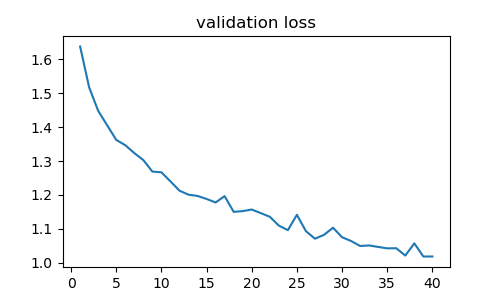
\includegraphics{base_validation_loss.png}
   \caption{\textbf{基础网络在测试集上的损失}}
\end{figure}
\begin{figure}[H]
   \centering
   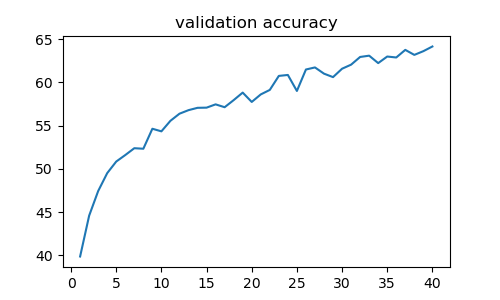
\includegraphics{base_validation_accuracy.png}
   \caption{\textbf{基础网络在测试集上的准确率}}
\end{figure}
可以看到,在经历40轮次的训练后,基础网络对cifar10数据集分类的准确率为64.14\%。

\section{个人实现的ResNet网络}
\subsection{网络结构}
\begin{lstlisting}[language = C++]
ResNet(
  (conv): Conv2d(3, 32, kernel_size=(7, 7), stride=(1, 1), padding=(3, 3))
  (bn): BatchNorm2d(32, eps=1e-05, momentum=0.1, affine=True, track_running_stats=True)
  (relu1): ReLU()
  (basic1): BasicBlock(
    (conv1): Conv2d(32, 32, kernel_size=(3, 3), stride=(1, 1), padding=(1, 1))
    (bn1): BatchNorm2d(32, eps=1e-05, momentum=0.1, affine=True, track_running_stats=True)
    (relu1): ReLU()
    (conv2): Conv2d(32, 32, kernel_size=(3, 3), stride=(1, 1), padding=(1, 1))
    (relu2): ReLU()
    (bn2): BatchNorm2d(32, eps=1e-05, momentum=0.1, affine=True, track_running_stats=True)
  )
  (basic2): BasicBlock(
    (conv1): Conv2d(32, 64, kernel_size=(3, 3), stride=(1, 1), padding=(1, 1))
    (bn1): BatchNorm2d(64, eps=1e-05, momentum=0.1, affine=True, track_running_stats=True)
    (relu1): ReLU()
    (conv2): Conv2d(64, 64, kernel_size=(3, 3), stride=(2, 2), padding=(1, 1))
    (relu2): ReLU()
    (bn2): BatchNorm2d(64, eps=1e-05, momentum=0.1, affine=True, track_running_stats=True)
    (sample): DownSample(
      (conv): Conv2d(32, 64, kernel_size=(1, 1), stride=(2, 2))
      (batch_normal): BatchNorm2d(64, eps=1e-05, momentum=0.1, affine=True, track_running_stats=True)
    )
  )
  (basic3): BasicBlock(
    (conv1): Conv2d(64, 64, kernel_size=(3, 3), stride=(1, 1), padding=(1, 1))
    (bn1): BatchNorm2d(64, eps=1e-05, momentum=0.1, affine=True, track_running_stats=True)
    (relu1): ReLU()
    (conv2): Conv2d(64, 64, kernel_size=(3, 3), stride=(1, 1), padding=(1, 1))
    (relu2): ReLU()
    (bn2): BatchNorm2d(64, eps=1e-05, momentum=0.1, affine=True, track_running_stats=True)
  )
  (basic4): BasicBlock(
    (conv1): Conv2d(64, 128, kernel_size=(3, 3), stride=(1, 1), padding=(1, 1))
    (bn1): BatchNorm2d(128, eps=1e-05, momentum=0.1, affine=True, track_running_stats=True)
    (relu1): ReLU()
    (conv2): Conv2d(128, 128, kernel_size=(3, 3), stride=(2, 2), padding=(1, 1))
    (relu2): ReLU()
    (bn2): BatchNorm2d(128, eps=1e-05, momentum=0.1, affine=True, track_running_stats=True)
    (sample): DownSample(
      (conv): Conv2d(64, 128, kernel_size=(1, 1), stride=(2, 2))
      (batch_normal): BatchNorm2d(128, eps=1e-05, momentum=0.1, affine=True, track_running_stats=True)
    )
  )
  (basic5): BasicBlock(
    (conv1): Conv2d(128, 128, kernel_size=(3, 3), stride=(1, 1), padding=(1, 1))
    (bn1): BatchNorm2d(128, eps=1e-05, momentum=0.1, affine=True, track_running_stats=True)
    (relu1): ReLU()
    (conv2): Conv2d(128, 128, kernel_size=(3, 3), stride=(1, 1), padding=(1, 1))
    (relu2): ReLU()
    (bn2): BatchNorm2d(128, eps=1e-05, momentum=0.1, affine=True, track_running_stats=True)
  )
  (fc1): Linear(in_features=8192, out_features=1024, bias=True)
  (fc2): Linear(in_features=1024, out_features=100, bias=True)
  (relu2): ReLU()
)
\end{lstlisting}
具体结构可以画草图如下
\begin{figure}[H]
   \centering
   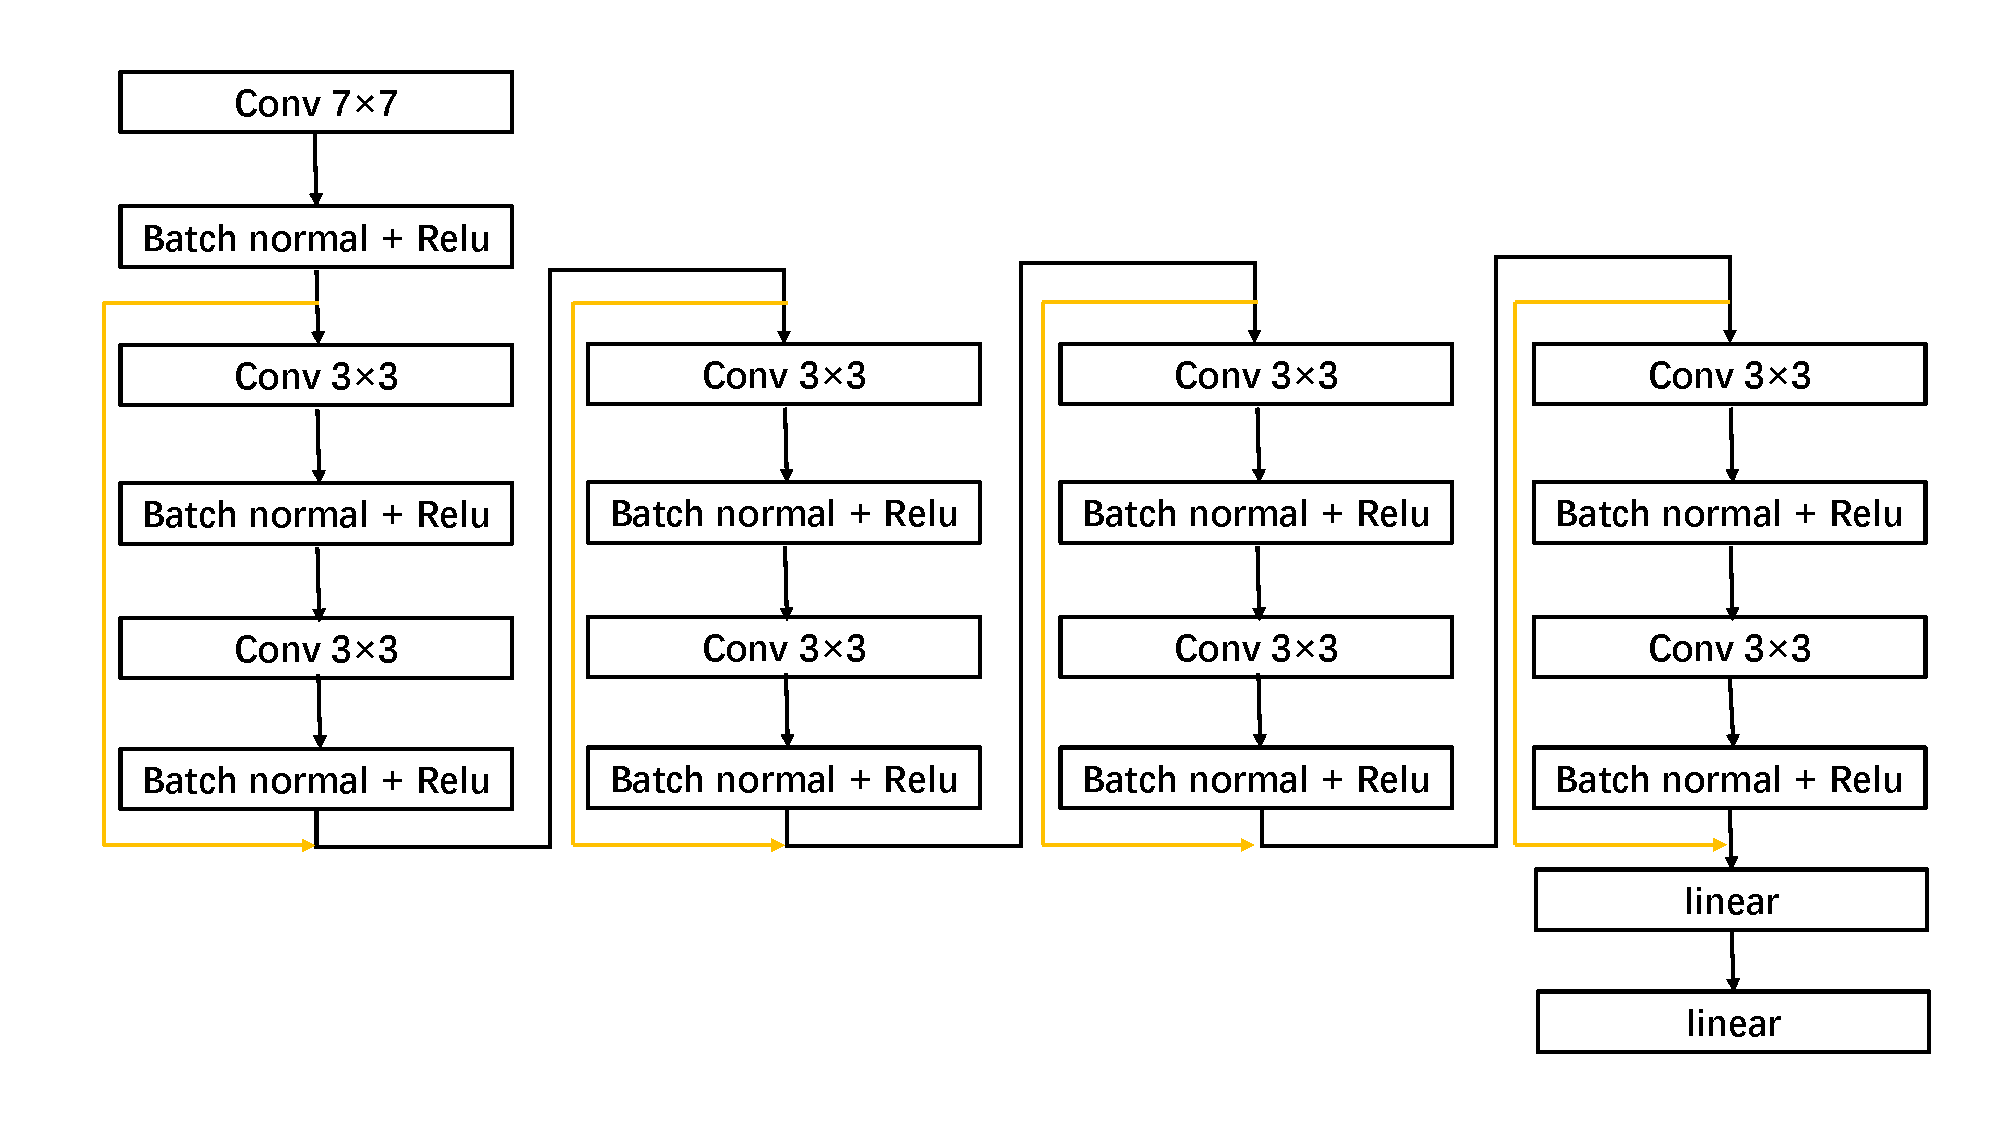
\includegraphics[scale= 0.3]{展示}

\end{figure}
\subsection{实验结果}
\begin{figure}[H]
   \centering
   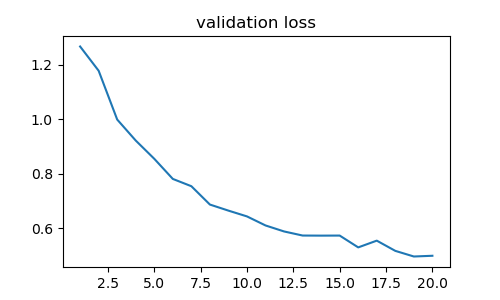
\includegraphics{Resnet_validation_loss.png}
   \caption{\textbf{个人实现的ResNet网路在测试集上的损失}}
\end{figure}
\begin{figure}[H]
   \centering
   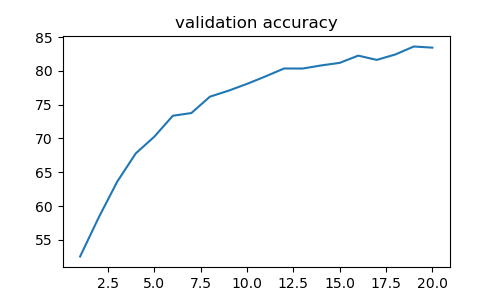
\includegraphics{Resnet_validation_accuracy.png}
   \caption{\textbf{个人实现的ResNet网路在测试集上的准确率}}
\end{figure}
可以看到,在经历40轮次的训练后,个人实现的ResNet对cifar10数据集分类的准确率为83.43\%。
\section{个人实现的DenseNet网络}
\subsection{网络结构}
我们根据Densely connected convolutional networks原文中描述的网络结构进行简单设计,因为计算力有限,所以只采用了两个DenseBlock和一个TransitionBlock。

\noindent 利用pycharm打印网络结构如下:
\begin{lstlisting}
DenseNet(
  (conv): Conv2d(3, 32, kernel_size=(7, 7), stride=(2, 2), padding=(3, 3))
  (bn1): BatchNorm2d(32, eps=1e-05, momentum=0.1, affine=True, track_running_stats=True)
  (max_pool): MaxPool2d(kernel_size=2, stride=2, padding=0, dilation=1, ceil_mode=False)
  (relu): ReLU()
  (denseblock1): DenseBlock(
    (denseblock): Sequential(
      (0): DenseBasic(
        (layer): Sequential(
          (0): BatchNorm2d(32, eps=1e-05, momentum=0.1, affine=True, track_running_stats=True)
          (1): ReLU()
          (2): Conv2d(32, 128, kernel_size=(1, 1), stride=(1, 1))
          (3): BatchNorm2d(128, eps=1e-05, momentum=0.1, affine=True, track_running_stats=True)
          (4): ReLU()
          (5): Conv2d(128, 32, kernel_size=(3, 3), stride=(1, 1), padding=(1, 1))
        )
      )
      (1): DenseBasic(
        (layer): Sequential(
          (0): BatchNorm2d(64, eps=1e-05, momentum=0.1, affine=True, track_running_stats=True)
          (1): ReLU()
          (2): Conv2d(64, 128, kernel_size=(1, 1), stride=(1, 1))
          (3): BatchNorm2d(128, eps=1e-05, momentum=0.1, affine=True, track_running_stats=True)
          (4): ReLU()
          (5): Conv2d(128, 32, kernel_size=(3, 3), stride=(1, 1), padding=(1, 1))
        )
      )
      (2): DenseBasic(
        (layer): Sequential(
          (0): BatchNorm2d(96, eps=1e-05, momentum=0.1, affine=True, track_running_stats=True)
          (1): ReLU()
          (2): Conv2d(96, 128, kernel_size=(1, 1), stride=(1, 1))
          (3): BatchNorm2d(128, eps=1e-05, momentum=0.1, affine=True, track_running_stats=True)
          (4): ReLU()
          (5): Conv2d(128, 32, kernel_size=(3, 3), stride=(1, 1), padding=(1, 1))
        )
      )
      (3): DenseBasic(
        (layer): Sequential(
          (0): BatchNorm2d(128, eps=1e-05, momentum=0.1, affine=True, track_running_stats=True)
          (1): ReLU()
          (2): Conv2d(128, 128, kernel_size=(1, 1), stride=(1, 1))
          (3): BatchNorm2d(128, eps=1e-05, momentum=0.1, affine=True, track_running_stats=True)
          (4): ReLU()
          (5): Conv2d(128, 32, kernel_size=(3, 3), stride=(1, 1), padding=(1, 1))
        )
      )
      (4): DenseBasic(
        (layer): Sequential(
          (0): BatchNorm2d(160, eps=1e-05, momentum=0.1, affine=True, track_running_stats=True)
          (1): ReLU()
          (2): Conv2d(160, 128, kernel_size=(1, 1), stride=(1, 1))
          (3): BatchNorm2d(128, eps=1e-05, momentum=0.1, affine=True, track_running_stats=True)
          (4): ReLU()
          (5): Conv2d(128, 32, kernel_size=(3, 3), stride=(1, 1), padding=(1, 1))
        )
      )
      (5): DenseBasic(
        (layer): Sequential(
          (0): BatchNorm2d(192, eps=1e-05, momentum=0.1, affine=True, track_running_stats=True)
          (1): ReLU()
          (2): Conv2d(192, 128, kernel_size=(1, 1), stride=(1, 1))
          (3): BatchNorm2d(128, eps=1e-05, momentum=0.1, affine=True, track_running_stats=True)
          (4): ReLU()
          (5): Conv2d(128, 32, kernel_size=(3, 3), stride=(1, 1), padding=(1, 1))
        )
      )
    )
  )
  (bn2): BatchNorm2d(224, eps=1e-05, momentum=0.1, affine=True, track_running_stats=True)
  (conv1): Conv2d(224, 64, kernel_size=(3, 3), stride=(1, 1), padding=(1, 1))
  (avg1): AvgPool2d(kernel_size=2, stride=2, padding=0)
  (denseblock2): DenseBlock(
    (denseblock): Sequential(
      (0): DenseBasic(
        (layer): Sequential(
          (0): BatchNorm2d(64, eps=1e-05, momentum=0.1, affine=True, track_running_stats=True)
          (1): ReLU()
          (2): Conv2d(64, 256, kernel_size=(1, 1), stride=(1, 1))
          (3): BatchNorm2d(256, eps=1e-05, momentum=0.1, affine=True, track_running_stats=True)
          (4): ReLU()
          (5): Conv2d(256, 64, kernel_size=(3, 3), stride=(1, 1), padding=(1, 1))
        )
      )
      (1): DenseBasic(
        (layer): Sequential(
          (0): BatchNorm2d(128, eps=1e-05, momentum=0.1, affine=True, track_running_stats=True)
          (1): ReLU()
          (2): Conv2d(128, 256, kernel_size=(1, 1), stride=(1, 1))
          (3): BatchNorm2d(256, eps=1e-05, momentum=0.1, affine=True, track_running_stats=True)
          (4): ReLU()
          (5): Conv2d(256, 64, kernel_size=(3, 3), stride=(1, 1), padding=(1, 1))
        )
      )
      (2): DenseBasic(
        (layer): Sequential(
          (0): BatchNorm2d(192, eps=1e-05, momentum=0.1, affine=True, track_running_stats=True)
          (1): ReLU()
          (2): Conv2d(192, 256, kernel_size=(1, 1), stride=(1, 1))
          (3): BatchNorm2d(256, eps=1e-05, momentum=0.1, affine=True, track_running_stats=True)
          (4): ReLU()
          (5): Conv2d(256, 64, kernel_size=(3, 3), stride=(1, 1), padding=(1, 1))
        )
      )
      (3): DenseBasic(
        (layer): Sequential(
          (0): BatchNorm2d(256, eps=1e-05, momentum=0.1, affine=True, track_running_stats=True)
          (1): ReLU()
          (2): Conv2d(256, 256, kernel_size=(1, 1), stride=(1, 1))
          (3): BatchNorm2d(256, eps=1e-05, momentum=0.1, affine=True, track_running_stats=True)
          (4): ReLU()
          (5): Conv2d(256, 64, kernel_size=(3, 3), stride=(1, 1), padding=(1, 1))
        )
      )
      (4): DenseBasic(
        (layer): Sequential(
          (0): BatchNorm2d(320, eps=1e-05, momentum=0.1, affine=True, track_running_stats=True)
          (1): ReLU()
          (2): Conv2d(320, 256, kernel_size=(1, 1), stride=(1, 1))
          (3): BatchNorm2d(256, eps=1e-05, momentum=0.1, affine=True, track_running_stats=True)
          (4): ReLU()
          (5): Conv2d(256, 64, kernel_size=(3, 3), stride=(1, 1), padding=(1, 1))
        )
      )
      (5): DenseBasic(
        (layer): Sequential(
          (0): BatchNorm2d(384, eps=1e-05, momentum=0.1, affine=True, track_running_stats=True)
          (1): ReLU()
          (2): Conv2d(384, 256, kernel_size=(1, 1), stride=(1, 1))
          (3): BatchNorm2d(256, eps=1e-05, momentum=0.1, affine=True, track_running_stats=True)
          (4): ReLU()
          (5): Conv2d(256, 64, kernel_size=(3, 3), stride=(1, 1), padding=(1, 1))
        )
      )
    )
  )
  (fc1): Linear(in_features=7168, out_features=10, bias=True)
)
\end{lstlisting}
\subsection{实验结果}
\begin{figure}[H]
  \centering
  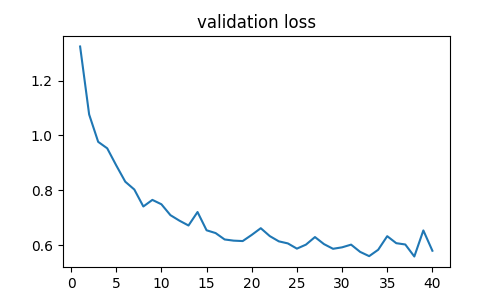
\includegraphics{validation_loss.png}
  \caption{\textbf{个人实现的DenseNet在测试集上的损失}}
\end{figure}
\begin{figure}[H]
  \centering
  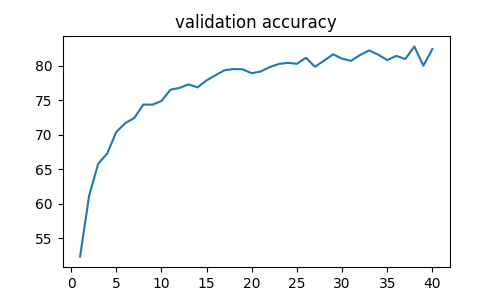
\includegraphics{validation_accuracy.png}
  \caption{\textbf{个人实现的DenseNet在测试集上的准确率}}
\end{figure}
可以看到,在经历40轮次的训练后,个人实现的DenseNet对cifar10数据集分类的准确率为82.82\%。

\section{解释没有跳跃连接的卷积网络、ResNet、DenseNet在训练过程中有什么不同}
\paragraph*{残差网络} 正如在[1]一文中指出的那样,残差网络是指在每两个卷积层之间,即几个特征抽取模块之间,加入了短路链接,这就是残差的由来,又称为恒等映射。这种操作可以将梯度之间传导给下一个模块块,避免了梯度消失的问题。于此同时,在训练的过程中某些卷积层可能已经达到了最优解,此时没有再进行训练的必要。通过这种操作,我们可以在接下来的训练中,直接跳过这两个卷积层,不会破坏之前训练出来的最优解。

\begin{figure}[H]
  \centering
  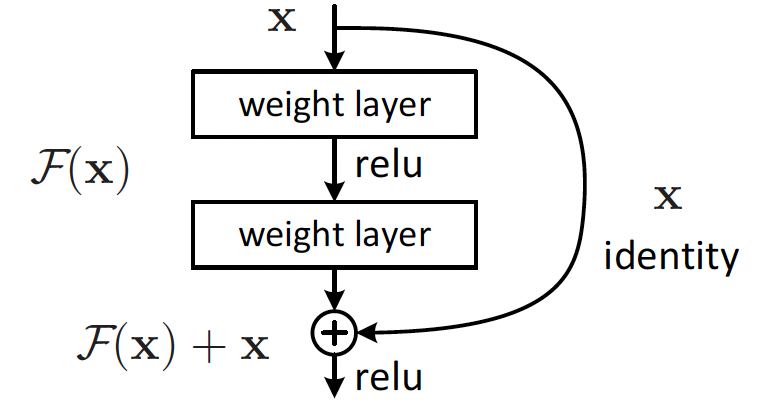
\includegraphics[scale = 0.4]{Resnet} 
  \caption{\textbf{基于ResNet的基础结构[1]}}
\end{figure}

$$
y = \mathcal{F} (x)+ x
$$
其中,$y$代表的是通过残差网络后输出的特征值,$x$代表的是输入的特征值,$\mathcal{F} $代表的是卷积操作。其中,有一些卷积改变了图像的形状,这时候我们需要对输入的残差连接进行下采样,具体就是用一个$1\times 1$的卷积,设置步长为2来改变残差的形状,使其可以顺利的与卷积层的输出进行相加。

\begin{figure}[H]
  \centering
  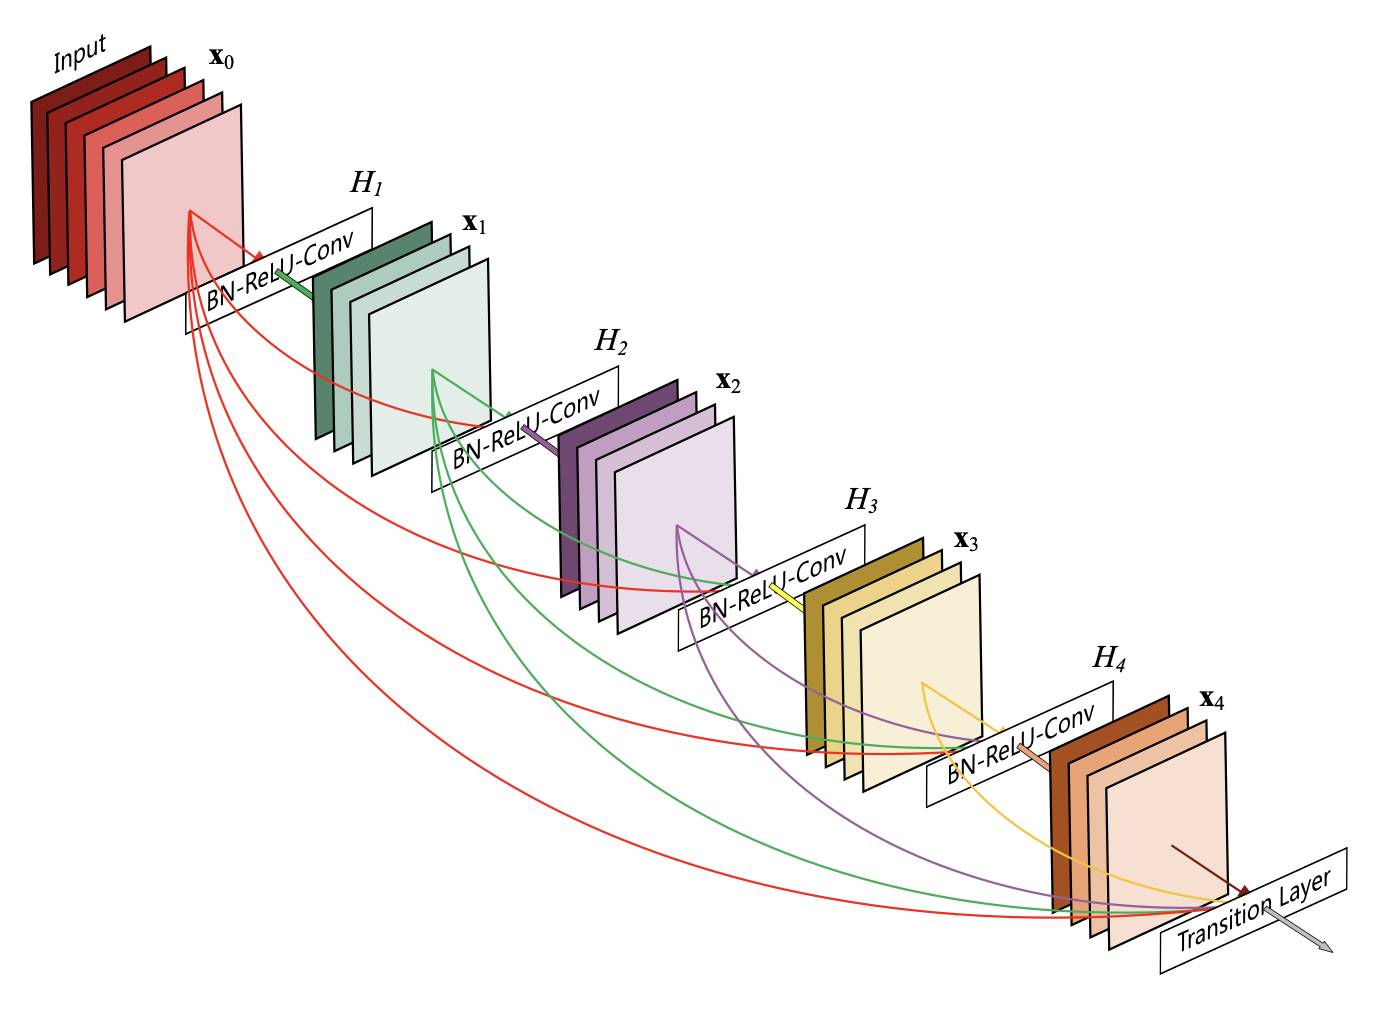
\includegraphics[scale = 0.4]{22} 
  \caption{\textbf{基于DesnsNet的基础结构[2]}}
\end{figure}

\paragraph*{DenseNet} 如[2]一文中所说,当前馈卷积神经网络的深度过深的时候,信息通过许多层后,可能会被消失或“洗掉”。在借鉴的思想之后,Denset也提出了一种残差结构,这种结构的每个层都从前面的层获得额外的输入,并将自己的特征图传递给所有后续层。这种与ResNet最大的不同是,ResNet是将残差和输出进行相加,而Desnet则是将输出和残差进行拼接。

由于不需要重新学习冗余的特征,这种操作比传统的卷积需要更少的参数。传统的卷积网络的堆叠可以看作是具有具有状态的算法,并在层与层之间传递,但与此同时也会将保留信息进行传递。ResNet可以通过残差使保留信息变得更加明确,并在训练中找出贡献非常小的层进行放弃,但参数量大大的增加。DenseNet的框架则明确区分了在训练过程中可以将每一层的保留信息和传递的信息进行区分,在与ResNet具有共同的优先时,DenseNet可以减少大量的参数量,且训练过程更加容易,过拟合的风险更小。



\section*{参考文献}
[1] K. He, X. Zhang, S. Ren, and J. Sun. Deep residual learning for image recognition. In Proceedings of the IEEE conference on computer vision and pattern recognition, pages 770–778, 2016

\noindent [2] G.Huang,Z.Liu,L.VanDerMaaten,andK.Q.Weinberger. Densely connected convolutional networks. In Proceedings of the IEEE conference on computer vision and pattern recognition, pages 4700–4708, 2017.

\end{document}
